\chapter{Database Structures}
\index{Database Structures}

\section{Overview}

This chapter describes the internal structures describing an IOC database.
It is of interest to EPICS system developers but serious application developers may also find it useful.
This chapter was intended to make it easier to understand the IOC source listings, but the information in it is likely to be outdated.
It also lists some of the header files provided for interfacing to IOC code.

\section{Include Files}

This section lists the files in base/include that are of most interest to IOC Application Developers:

\begin{description}

\item[alarm.h] - Definitions for alarm status and severity values.

\item[callback.h] - The definitions for the General Purpose callback system.

\item[dbAccess.h] - Definitions for the runtime database access routines.

\item[dbBase.h] - Definitions for the structures used to store an EPICS database.

\item[dbDefs.h] - A catchall file for definitions that have no other reasonable place to appear.

\item[dbFldTypes.h] - Definitions for \verb|DBF_xxx| and \verb|DBR_xxx| types.

\item[dbScan.h] - Definitions for the scanning system.

\item[dbStaticLib.h] - The static databases access system.

\item[db\_access.h db\_addr.h] - Old database access.

\item[devLib.h] - The device support library

\item[devSup.h] - Device Support Modules

\item[drvSup.h] - Driver Support Modules

\item[initHooks.h] - Definitions used by \verb|initHooks.c| routines.

\item[link.h] - Link definitions

\item[recSup.h] - The record global routines.

\item[special.h] - Definitions for special fields, i.e. \verb|SPC_xxx|.

\item[taskwd.h] - Task Watchdog System

\end{description}

\newpage

\section{Structures}

\begin{center}

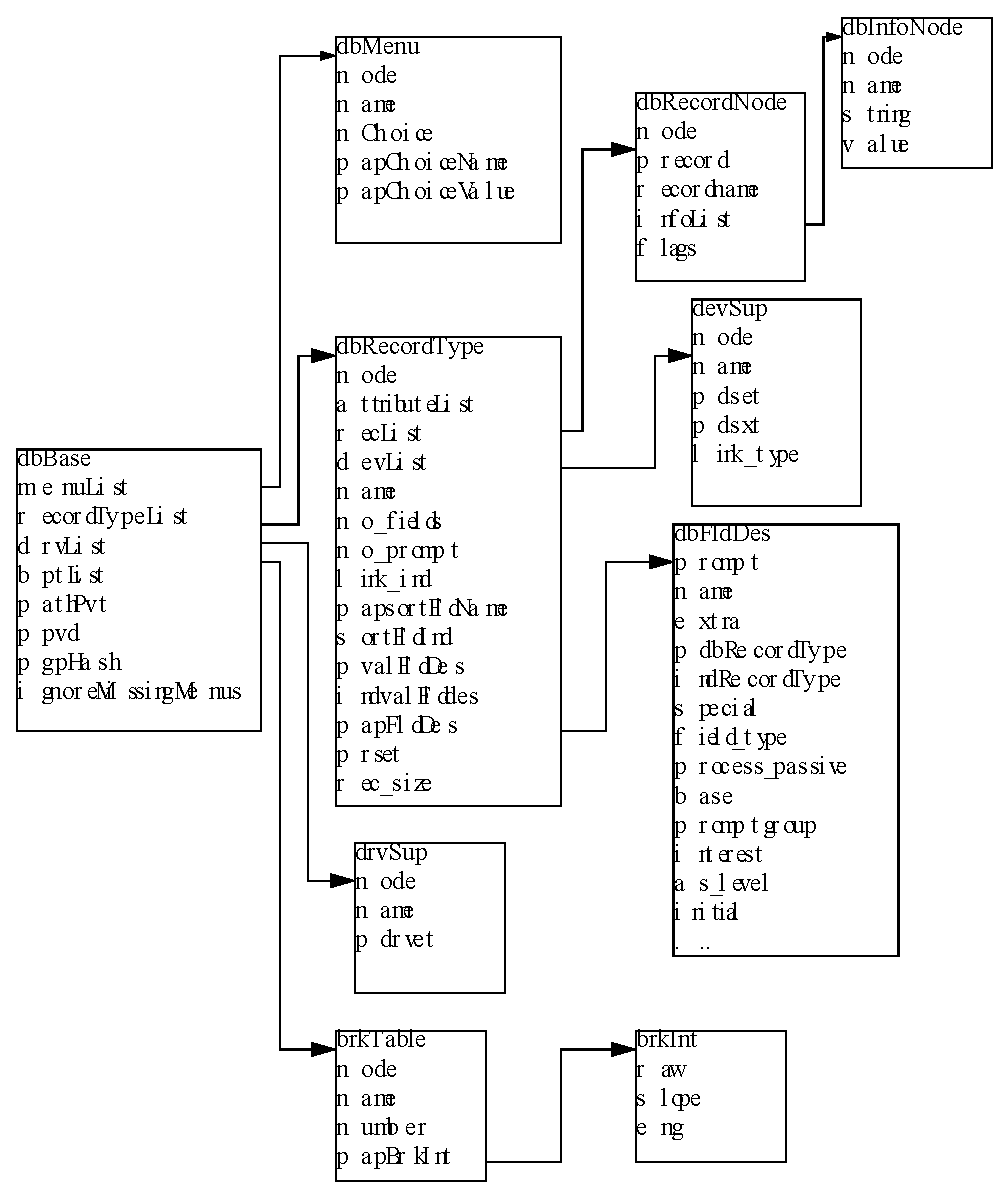
\includegraphics{databaseStructures_1}

\end{center}
